\section{Task Definition}
\label{sec:task}
%The temporally ordered user interactions lead to the streaming nature of session data. Therefore it's natural and realistic to formulate the news recommendation task as a session-based recommendation task to predict next-item. 
Assume that an anonymous user $u$ produces a sequence of click
events $S_u$ with length $T$, which can be represented as \[S_u: (n_1^u)\rightarrow(n_2^u)\rightarrow...\rightarrow(n_i^u)\rightarrow...,\]
where $n_i^u$ denotes the id of the $i$-th clicked article. 

In the training phase, the recommendation system aims to model the 
user feedback sequence as vector $\mathbf{x_s}$, 
maximizing the similarity between
the vector of predicted next-article ($n_{i+1}^u$) and $\mathbf{x_s}$. 
While in the test phase, 
given interaction sequence $S_u$ as input, 
we produce a ranking list $R$ with the probability that the target user $u$ is likely to click next from high to low. 
Typically a recommender needs to recommend more
than one item for a user, thus the top-k items in $R$ are recommended.
Note that in our anonymous settings, each user $u$ only appears once, 
which means training set and test set do not share the same users. 

\tabref{tb:note} summarizes some critical symbols and notations we use, 
and in later sections, for brevity, we ignore the superscript $u$ 
when discussing the information for a particular user. To explain further, the set $Imp_u$ denotes the articles in the vicinity of the articles
being clicked, which may have left an impression on the user.


\begin{table}[t]
    \caption{Notations and descriptions}
    \begin{tabular}{l|l}
    \toprule
    Symbol & Description\\
    \midrule
    $S_u$ & A session produced by an anonymous user $u$.\\
    $T$ & The number of articles in $S_u$.\\
    $i$ & $i\in [1,T]$ indexes articles in $S_u$.\\ 
    $n_i$ & The id of $i$-th article clicked by $u$.\\
    $\mathbf{c}_i$ & The Content representation of the article $n_i$ in $S_u$ \\
    $t_i$ & The active time that $u$ stays in the article $n_i$. \\
    $\mathbf{ta}_i$ & The encoded active duration that $u$ stays in $n_i$. \\
    $\mathbf{ts}_i$ & The encoded click time that $u$ click for article $n_i$. \\
    $\mathbf{tp}_i$ & The encoded publishing time of article $n_i$. \\
    $Imp_u$ & A set of articles that appear in $u$'s impression list.\\
    $\mathbf{x}_i$ & The item embedding vector of $n_i$.\\
    $\mathbf{xc}_i$ & The embedding vector of $n_i$ combined  $\mathbf{x}_i$ and $\mathbf{c}_i$.\\
    $\mathbf{xc_s}$ & The contextual session vector of $S_u$.\\
    $\mathbf{xt_s}$ & The temporal session vector of $S_u$.\\
    $\mathbf{x_s}$ & The final session vector of $S_u$.\\
    $N$ & The total number of articles.\\
    $j$ & $j\in [1,N]$ indexes total $N$ articles and is article id.\\
    $\hat{y_j}^u$ & The score of article $j$ clicked by $u$ in the next step.\\
    $R$ & Ranking list generated according to $\hat{y_j}^u$.\\
    $Ne_u$ & The set of negative samples for each $S_u$.\\
    \bottomrule
    \end{tabular}
    \label{tb:note}
\end{table}

% The whole procedure is depicted in \figref{fig:task}.

% \begin{figure}[th]
%     \centering
%     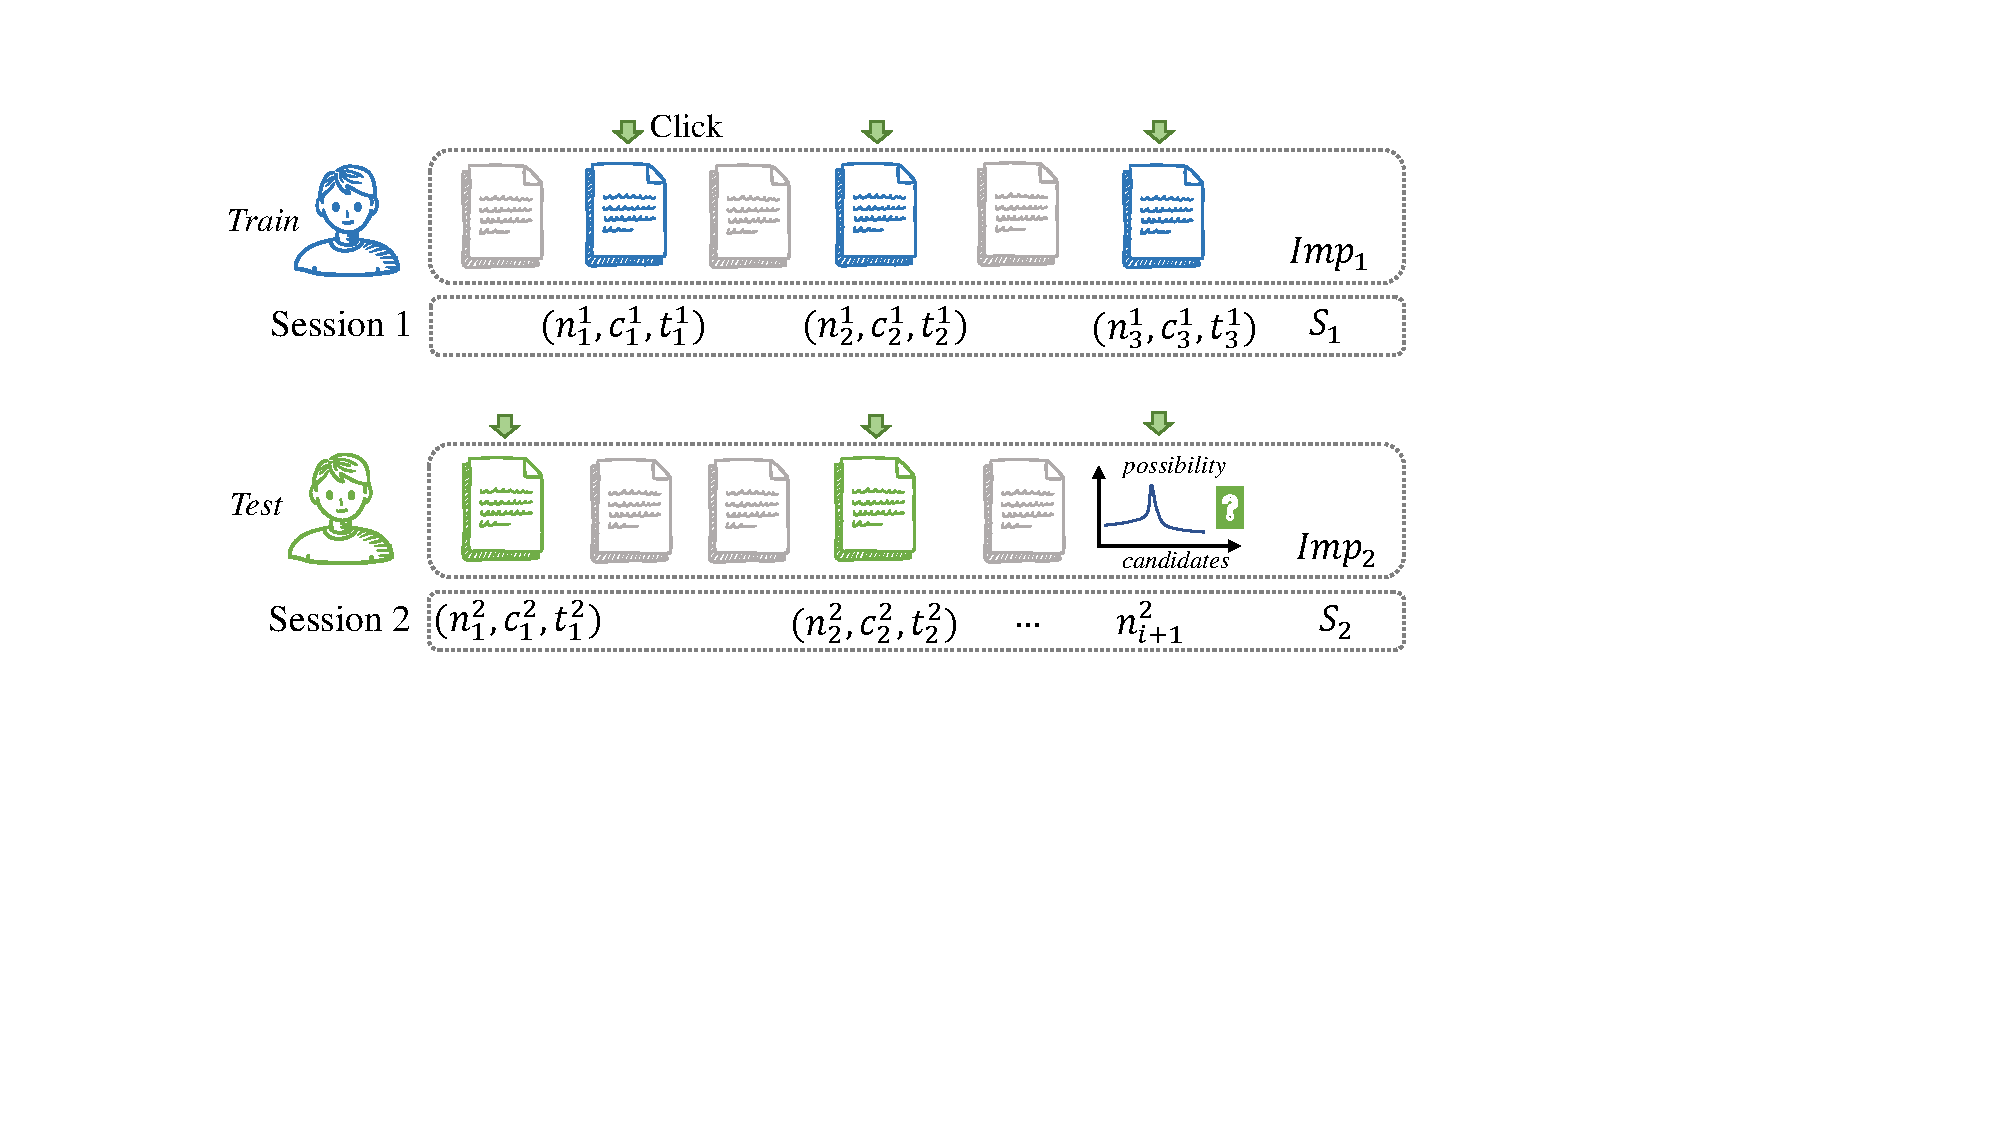
\includegraphics[width=\columnwidth]{fig/task.pdf}
%     \caption{Session-based news recommendation procedure.}
%     \label{fig:task}
% \end{figure}
